\documentclass{aip-cp}

\usepackage[numbers]{natbib}
\usepackage{rotating}
\usepackage{graphicx}
\usepackage{subcaption}

% \usepackage{amsmath,amsthm} 
% \usepackage{amsfonts}
% \usepackage{auto-pst-pdf} 

%\makeatletter
%\def\@fnsymbol#1{\ensuremath{\ifcase#1\or *\or \dagger\or **\or
%   \ddagger\or \mathsection\or \mathparagraph\or \|\or \dagger\dagger
%   \or \ddagger\ddagger \or\mathsection\mathsection
%   \or \mathparagraph\mathparagraph \or *{*}*\or
%   \dagger{\dagger}\dagger \or\ddagger{\ddagger}\ddagger\or
%   \mathsection{\mathsection}\mathsection
%   \or \mathparagraph{\mathparagraph}\mathparagraph \else\@ctrerr\fi}}
%\makeatother

% Document starts
\begin{document}

% Title portion
\title{Investigation on Minimal Hamiltonian for System of Material with Highly Anisotropic Transport and Optical Properties}

% \author[aff1]{Bayu Aditya\noteref{note1,note2}}
\author{Bayu Aditya}
\author{Muhammad Aziz Majidi\corref{cor1}}

\affil{Department of Physics, Faculty of Mathematics and Natural Sciences, Universitas Indonesia, Kampus UI Depok, Indonesia}
\corresp[cor1]{Corresponding author: aziz.majidi@sci.ui.ac.id}
% \authornote[note1]{This is an example of first authornote.}
% \authornote[note2]{This is an example of second authornote.}

\maketitle


\begin{abstract}
In a study at the Department of Physics, National University Singapore (NUS) of $\mathrm{Sr_{1-y}NbO_{3+\delta}}$ material revealed that the material has very high anisotropic characteristics, which are conductors in the a-axis, and insulators in the b and c crystal axis. This happens because of the contribution of orbitals to certain atoms that make the material anisotropic. To find out the contributing orbitals, we reconstruct the multi-band tight-binding Hamiltonian and reduce the orbitals that have a low contribution in around the fermi level, so that we will get a minimal Hamiltonian that has anisotropic characteristics. The results show that the d-orbitals of Nb atoms in the interfaces, O atoms between Nb and the crystal structure of $\mathrm{SrNbO_{3,4}}$ itself have a contribution to the material so that they are anisotropic.
\end{abstract}

% Head 1
\section{INTRODUCTION}
Strontium Niobates with type $\mathrm{SrNbO_{3.4}} $ has an interesting thing to study because of its structure and physical property \cite{andrivo}. Material $\mathrm{SrNbO_{3.4}}$ is a derivative of the compound $\mathrm{SrNbO_{3}}$ in the presence of additional oxygen, separated by octahedra $\mathrm{NbO_{6}}$ in the direction of $\{110\}$ \cite{LICHTENBERG2001,LICHTENBERG2008}. Due to the addition of oxygen, the material forms an interface which greatly influences the occupancy of Nb electrons in the d-orbitals \cite{chen}.

Previous research revealed that the material $\mathrm{SrNbO_{3,4}} $ has high anistropic properties, which have the characteristics of conductors and insulators in different crystal axis directions \cite{andrivo}. Because of these characteristics, this material can be developed as optically-controlled switches on the basis of logic operations in electronic circuits.

This motivates us to understand what causes the material to have very high anisotropic characteristics. So with this understanding, it can be predicted that other materials can produce similar characteristics.

\begin{figure}[b]
  \centerline{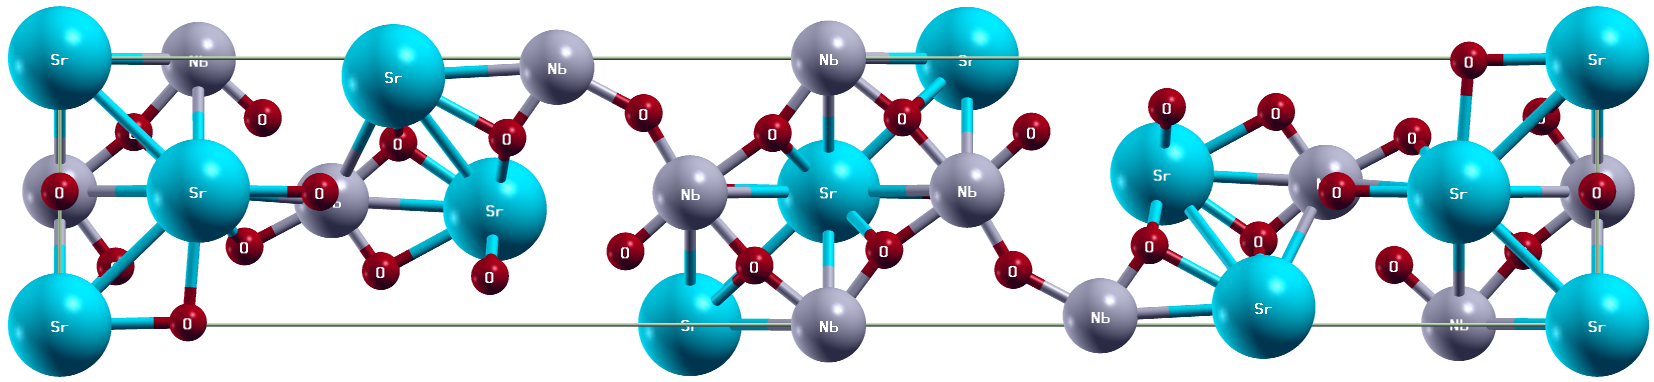
\includegraphics[width=200pt]{graph/pwi2xsf.png}}
  \caption{Crystal structure $\mathrm{SrNbO_{3,4}}$. Sr atoms are marked in blue, Nb atoms are marked in gray, O atoms are marked in red. There is a distance that is tenuous and forms 3 groups (left, center, right) separated with interfaces due to the addition of oxygen atoms.}
\end{figure}

\section{MODEL}
the material we use to investigate anisotropic characteristics is $\mathrm{SrNbO_{3.4}}$. This material is a derivative of compound $\mathrm{SrNbO_{3}}$. The difference between $\mathrm{SrNbO_{3}} $ and $ \mathrm{SrNbO_{3,4}} $ is that there are additional oxygen atoms in every 5 layers \cite {Wan2017}. Because there is additional oxygen, there is a tenuous distance and forms 3 groups on the left, center and right side separated with interfaces (Fig 1).

We model our $\mathrm{SrNbO_{3,4}}$ material system with the equation of multi-band Tight-Binding Hamiltonian approximation,
$$ H_{ij}(\vec{k}) = \frac{1}{N}\sum_{nm}\sum_{\alpha \beta}e^{-i\vec{k} \cdot (\vec{r}_{in}-\vec{r}_{jm})} t_{in\alpha, jm\beta} $$

\begin{figure}[t]
  \centerline{\includegraphics[width=200pt,angle=-90]{graph/band_dos_qe_23x3x17.eps}}
  \caption{Band Structure and Density of States from First Principle Calculation Using Quantum Espresso}
\end{figure}

assuming electron hopping from orbitals $i$ to $j$, atom $n$ to $m$, and unit cell $\alpha$ to $\beta$ as many as N unit cell. Position of electron in orbitals $i$ and atom $n$ located in $r_{in}$, and electron in orbitals $j$ and atom $m$ located in $r_{jm}$. The momentum that the electron is equal to $\vec{k}$. While $t_{in\alpha, jm\beta}$ is a hopping parameter in the electrons.

\begin{figure}[b]
  \centerline{\includegraphics[width=200pt]{graph/band_TB_original.eps}}
  \caption{Band Structure from Hamiltonian Tight-Binding Multiband.}
\end{figure}

In this paper, we model the material with several types of orbitals that are considered valence electrons. Like the Strontium (Sr) atom have $ 4s-5s-4p-5p $ orbitals, Niobium (Nb) atoms have $ 4s-5s-4p-5p-4d $ orbitals, and Oxygen (O) atoms have $ 2s-2p $ orbitals . The material that we use has 10 Strontium atoms, 10 Niobium atoms, and 34 Oxygen \cite{persson} atoms. So there are 346 types of valence electron orbitals that we use.

\section{METHOD}
In the initial stage, we performed the first-principle calculation by calculating the density functional theory (DFT) and maximally-localized wannier function (MLWFs). For DFT calculations, we use the Quantum Espresso package \cite{QE-2017, QE-2009}. While for the MLWFs calculation, we use the Wannier90 package \cite{wannier}. DFT calculation is doing to get a complete electronic structure of all valence orbitals of each atom. Furthermore, the results of this calculation continued with the MLWFs calculation to get the tight-binding parameter. From these parameters, we will use to construct the tight-binding multiband Hamiltonian matrix.

From the tight-binding Hamiltonian matrix, we doing the calculation of the eigenvalues to get the band-structure of the tight-binding approximation. and calculation the density of states using the green function. The green function equation used is,
$$ [G(\omega, \vec{k})] = \frac{1}{(\omega + i0^{+})[I] - [H(\vec{k})]} $$
From this green function can be used to determine partial density of state (PDOS) by using,
$$ PDOS_\alpha(\omega) = -\frac{1}{\pi}Im\sum_k{[G_{\alpha \alpha}(\omega, \vec{k})]} $$
and also total density of states (DOS) by using,
$$ DOS (\omega) = \sum_\alpha{PDOS_\alpha(\omega)}$$

\begin{figure}[t]
  \centerline{\includegraphics[width=200pt]{graph/dos_qetb.eps}}
  \caption{Comparison Density of States between First Principle Calculation and Tight Binding Calculations.}
\end{figure}

\section{RESULT AND DISCUSSION}
The first-principle calculation of the material $ \mathrm{SrNbO_{3,4}} $ produces a graph of the band structure which has an anisotropic structure. It can be seen in Figure 2 that for the a-axis ($ \mathrm{X - \Gamma} $) has conductor properties, while for the b-axis ($ \mathrm{\Gamma - Y} $) and c-axis ($ \mathrm{\Gamma-Z} $) has insulator properties. In this calculation, the Fermi level is set based on previous experimental data from angular-resolved photoemission spectroscopy (ARPES) \cite{kuntscher}.

The results of calculations using the tight-binding approximation show that the band structure in Figure 3 is the same as the first-principle calculation (fig 2). Similarly, the density of states in Figure 4 shows that the results of calculations using the tight-binding and first principle are the same. This shows that only using the tight-binding approximation is sufficient to produce the same physical properties in accordance with first-principle calculations.

We reduced the Hamiltonian tight binding matrix by removing orbitals that have no contribution in the energy range of 3 to 13.5 eV. Because in that energy range there are many electrons occupying, and also that energy range is located around the fermi level. To see which orbitals do not have a contribution in that energy range, we use a partial density of states (PDOS) calculation for each orbital and eliminate those that have low values ​​in that energy range.

From total 346 valence electron orbitals, we reduced 133 orbitals that had no electron contribution in that frequency range. The results of the band structure after the orbitals are reduced can be seen in Figure 5. In that picture, it can be seen that the material can still maintain anisotropic characteristics as before.

Based on PDOS calculations with DFT shows that around the fermi level is dominated by d-orbitals on the Nb atom \cite{Wan2017}. And also in the reduction of Tight Binding Hamiltonian previously found that there are several Nb atoms where the d-orbitals dominate in the area around the fermi level. The Nb atom located in the interfaces formed due to additional oxygen from $ \mathrm{SrNbO_{3}} $ to $ \mathrm{SrNbO_{3,4}} $ (fig 1). In addition, some oxygen atoms that are between Nb atoms also have a contribution around the fermi level.

\begin{figure}[t]
  \centerline{\includegraphics[width=280pt]{graph/TB_bands.eps}}
  \caption{Band Structure after Orbitals Reduction from Hamiltonian Tight-Binding Multiband.}
\end{figure}

We have not been able to reduce more than 133 orbitals because if more than these orbitals are reduced, the band structure that makes the characteristics of the material become anisotropic will collapse. So it can be said that in addition to the contributions of the Nb and O atoms previously described, the crystal structure of $ \mathrm{SrNbO_{3,4}} $ itself also has a strong contribution to its anisotropic characteristic.

\section{CONCLUSION}
We have already explained about $\mathrm{SrNbO_{3,4}}$ materials that have anisotropic characteristics using the tight-binding approximation. To find out which orbitals contribute to their anisotropic characteristics, we reduce non-contributing orbitals in the $ 3-13.5$ eV frequency range. We found that the d-orbitals on Nb at the interfaces, O atoms between Nb atoms, and the crystal structure of $ \mathrm{SrNbO_{3,4}} $ itself makes this material have anisotropic characteristics.

% Sections that will go in second font

% Acknowledgement
\section{ACKNOWLEDGMENTS}
We are very grateful to Universitas Indonesia for providing us a full funding for this project through PITTA B Research Grant No. NKB-0644/UN2.R3.1/HKP.05.00/2019. The computation in this work has been done using the facilities of HPC LIPI,
Indonesian Institute of Sciences (LIPI)

% References

\nocite{*}
\bibliographystyle{unsrt}%
\bibliography{work_eng}%


\end{document}